\newcommand{\scipy}{\texttt{scipy}\xspace}

\section{Examples}
\label{sec:MolsturmExamples}

In this section we present a few examples,
which demonstrate how the \python interface of \molsturm
could be combined with existing features of \python
in order to analyse results or to extend the capabilities of \molsturm.
In all cases shown the computations are done using contracted
Gaussian basis sets.
It should be noted, however,
that due to the basis-function-independent nature of \molsturm
the procedures outlined in the scripts could be easily used
with other types of basis functions as well.

\subsection{Fitting a dissociation curve}
\label{sec:ex:data}

\newcommand{\ldict}{59--63\xspace}
\newcommand{\lcall}{64\xspace}
\newcommand{\lextract}{34\xspace}

\begin{figure}
	\centering
	\begin{minipage}{0.58\textwidth}
	\lstinputlisting{examples/dissociation/h2_dissociation.py}
	\end{minipage}
	\caption[\python script computing a \ce{H2} dissociation curve]{
		Script for computing a \ce{H2} dissociation curve
		and fitting a Morse potential to it.
		The decision about the basis function type, the integral back end
		as well as the basis set are only made in line \lcall,
		where the \texttt{compute\_curve} is called with the chosen
		set of parameters.
	}
	\label{fig:codeDissociation}
\end{figure}

\begin{figure}
	\centering
	\includeimage[scale=0.8]{8_molsturm/h2_dissociation}
	\caption[Result from calling the python script of figure \ref{fig:codeDissociation}]{
		Plot resulting from computing the \ce{H2}
		dissociation curve in a def2-SVP basis set~\cite{Weigend2005}
		at UMP2 level,
		employing the script of figure \ref{fig:codeDissociation}.
		Shown are both the UMP2 energy values as well as the fitted
		Morse potential.}
	\label{fig:dissociation}
\end{figure}

Many day-to-day tasks in quantum chemistry boil down to
performing a multitude of similar calculations,
followed by a subsequent graphical analysis
by plotting or fitting.
Here we want to consider the computation of a dissociation curve
followed by the fit of a Morse potential
as an example for such a procedure.

Even though many traditional quantum-chemistry programs
have developed functionality for automatising simple
energy versus geometry scans,
the vast number of possible post-processing methodologies
makes it impossible to cover everything.
In other words in many cases one is required to write a script
to parse the program's output and then feed it to potentially yet
another program for doing the fitting and the plotting.

This has the disadvantage,
that skill in at least two different settings is required:
The domain-specific language the quantum-chemistry program uses
in its input file as well as the scripting language to parse the results.
For people who are new to the field this can become quite an obstacle.
More subtly the output formats
of quantum-chemistry programs change from time to time
breaking the parser scripts or --- even worse ---
producing wrong results without any notice.
This is a common problem in the practice of computational chemistry.

Contrast this with the approach taken by packages like \molsturm,
which can be controlled solely by a scripting language interface.
The \python script shown in figure \ref{fig:codeDissociation} performs
exactly what has been discussed above:
First, in the function \texttt{compute\_curve},
it computes the energy of the \ce{H2} molecule
at various bond distances using spin-unrestricted
second-order Møller-Plesset perturbation theory~(UMP2).
\todo{cite}
Then it calls the function \texttt{plot\_morse\_fit}
to plot the resulting data points of energies vs. distances
and to fit a Morse potential through them,
see figure \ref{fig:dissociation}.
Note, how the error-prone parsing step is replaced by just
line \lextract of figure \ref{fig:codeDissociation},
where UMP2 ground state energy is requested from the
dictionary of results returned by the calculation.

Since we are able to orchestrate the full computational procedure
from a single script,
all parameters influencing the computation, the plotting or the fitting
are denoted in a single location.
The script therefore serves as automatic documentation
of the precise computational procedure.
On top of that if our efforts are to be reproduced by someone else,
all it takes is to re-run the script.

It should be noted
that the present script only makes a single reference to the
parameters used for the selection of the discretisation basis,
namely in lines \ldict.
By a trivial extension one may hence utilise
this script as a building block for a systematic study
investigating the effect
a change of basis set, integral implementation or basis function type
might have on the UMP2 description of the \ce{H2}-dissociation.
Additionally the basis-function independent design of \molsturm
assures that if a new basis type or a new integral back end
becomes available in \gint,
only the appropriate keyword needs to be replaced in lines \ldict
in order to employ it for the UMP2 calculations instead.

\subsection{Coupled-cluster doubles}
\label{sec:ex:ccd}

\begin{sidewaysfigure}
	\colorlet{CcRes}{mauve}
\colorlet{CcEri}{green!35!black}
\colorlet{CcTOne}{blue!90!black}
\colorlet{CcTTwo}{orange!85!green!85!black}
\colorlet{CcFock}{red!75!orange!85!black}

\begin{minipage}{0.43\textwidth}
\newcommand{\ccfock}[1]{\textcolor{CcFock}{f_{#1}}}
\newcommand{\cctone}[2]{\textcolor{CcTOne}{t_{#1}^{#2}}}
\newcommand{\ccttwo}[2]{\textcolor{CcTTwo}{t_{#1}^{#2}}}
\newcommand{\cceri}[2]{\textcolor{CcEri}{\textcolor{CcEri}{\langle #1 || #2 \rangle}}}
\smaller
\vspace{1.0cm}
\begin{align*}
	\textcolor{CcRes}{r_{ij}^{ab}}
		&= \cceri{ab}{ij} \\
		%
		&+ \sum_e \ccfock{ae} \, \cctone{ij}{eb}
		 - \sum_e \ccfock{be} \, \cctone{ij}{ea}
		 - \sum_m \ccfock{mi} \, \cctone{mj}{ab}
		 + \sum_m \ccfock{mj} \, \cctone{mi}{ab} \\
		%
		&+ \frac12 \sum_{mn} \cceri{mn}{ij} \, \cctone{mn}{ab}
		+ \frac12 \sum_{ef} \cceri{ab}{ef} \, \cctone{ij}{ef} \\
		%
		&+ \sum_{me} \cceri{mb}{ej} \, \cctone{im}{ae}
		 - \sum_{me} \cceri{mb}{ei} \, \cctone{jm}{ae} \\
		&- \sum_{me} \cceri{ma}{ej} \, \cctone{im}{be}
		 + \sum_{me} \cceri{ma}{ei} \, \cctone{jm}{be} \\
		%
		&- \frac12 \sum_{mnef} \cceri{mn}{ef} \, \cctone{mn}{af} \, \ccttwo{ij}{eb}
		 + \frac12 \sum_{mnef} \cceri{mn}{ef} \, \cctone{mn}{bf} \, \ccttwo{ij}{ea} \\
		&- \frac12 \sum_{mnef} \cceri{mn}{ef} \, \cctone{in}{ef} \, \ccttwo{mj}{ab}
		 + \frac12 \sum_{mnef} \cceri{mn}{ef} \, \cctone{jn}{ef} \, \ccttwo{mi}{ab} \\
		&+ \frac14 \sum_{mnef} \cceri{mn}{ef} \, \cctone{mn}{ab} \, \ccttwo{ij}{ef}
		 + \frac12 \sum_{mnef} \cceri{mn}{ef} \, \cctone{im}{ae} \, \ccttwo{jn}{bf} \\
		&- \frac12 \sum_{mnef} \cceri{mn}{ef} \, \cctone{jm}{ae} \, \ccttwo{in}{bf}
		 - \frac12 \sum_{mnef} \cceri{mn}{ef} \, \cctone{im}{be} \, \ccttwo{jn}{af} \\
		&+ \frac12 \sum_{mnef} \cceri{mn}{ef} \, \cctone{jm}{be} \, \ccttwo{in}{af}
\end{align*}
\end{minipage}%
\hspace{0.2cm}
%
\begin{minipage}{0.50\textwidth}
\newcommand{\vvoo}{\textcolor{CcEri}{vvoo}}
\newcommand{\oovv}{\textcolor{CcEri}{oovv}}
\newcommand{\ovvo}{\textcolor{CcEri}{ovvo}}
\newcommand{\oooo}{\textcolor{CcEri}{oooo}}
\newcommand{\vvvv}{\textcolor{CcEri}{vvvv}}
\newcommand{\fvv}{\textcolor{CcFock}{state.fock.block("vv")}}
\newcommand{\foo}{\textcolor{CcFock}{state.fock.block("oo")}}
\newcommand{\eriIdx}{\textcolor{CcEri}{mnef}}
\newcommand{\tampOne}{\textcolor{CcTOne}{t2}}
\newcommand{\tampTwo}{\textcolor{CcTTwo}{t2}}
\newcommand{\resIdx}{\textcolor{CcRes}{iajb}}
\begin{BVerbatim}[commandchars=\\\{\},fontsize={\smaller}]
eri_phys = state.eri.transpose((0, 2, 1, 3))
eri = eri_phys - eri_phys.transpose((1, 0, 2, 3))
...

{\color{CcEri}oooo = eri.block("oooo"); vvvv = eri.block("vvvv")}
{\color{CcEri}oovv = eri.block("oovv"); ovvo = eri.block("ovvo")}
{\textcolor{CcRes}{res}} = (
    + np.einsum("{\color{CcEri}abij}->{\resIdx}", {\color{CcEri}eri.block("vvoo")})
    + np.einsum("{\color{CcFock}ae},{\color{CcTOne}iejb}->{\resIdx}", {\fvv}, {\tampOne})
    - np.einsum("{\color{CcFock}be},{\color{CcTOne}ieja}->{\resIdx}", {\fvv}, {\tampOne})
    - np.einsum("{\color{CcFock}mi},{\color{CcTOne}majb}->{\resIdx}", {\foo}, {\tampOne})
    + np.einsum("{\color{CcFock}mj},{\color{CcTOne}maib}->{\resIdx}", {\foo}, {\tampOne})

    + 0.5 * np.einsum("{\color{CcEri}mnij},{\color{CcTOne}manb}->{\resIdx}", {\oooo}, {\tampOne})
    + 0.5 * np.einsum("{\color{CcEri}abef},{\color{CcTOne}iejf}->{\resIdx}", {\vvvv}, {\tampOne})
    + np.einsum("{\color{CcEri}mbej},{\color{CcTOne}iame}->{\resIdx}", {\ovvo}, {\tampOne})
    - np.einsum("{\color{CcEri}mbei},{\color{CcTOne}jame}->{\resIdx}", {\ovvo}, {\tampOne})
    - np.einsum("{\color{CcEri}maej},{\color{CcTOne}ibme}->{\resIdx}", {\ovvo}, {\tampOne})
    + np.einsum("{\color{CcEri}maei},{\color{CcTOne}jbme}->{\resIdx}", {\ovvo}, {\tampOne})

    - 0.5  * np.einsum("{\eriIdx},{\color{CcTOne}manf},{\color{CcTTwo}iejb}->{\resIdx}", {\oovv}, {\tampOne}, {\tampTwo})
    + 0.5  * np.einsum("{\eriIdx},{\color{CcTOne}mbnf},{\color{CcTTwo}ieja}->{\resIdx}", {\oovv}, {\tampOne}, {\tampTwo})
    - 0.5  * np.einsum("{\eriIdx},{\color{CcTOne}ienf},{\color{CcTTwo}majb}->{\resIdx}", {\oovv}, {\tampOne}, {\tampTwo})
    + 0.5  * np.einsum("{\eriIdx},{\color{CcTOne}jenf},{\color{CcTTwo}maib}->{\resIdx}", {\oovv}, {\tampOne}, {\tampTwo})
    + 0.25 * np.einsum("{\eriIdx},{\color{CcTOne}manb},{\color{CcTTwo}iejf}->{\resIdx}", {\oovv}, {\tampOne}, {\tampTwo})
    + 0.5  * np.einsum("{\eriIdx},{\color{CcTOne}iame},{\color{CcTTwo}jbnf}->{\resIdx}", {\oovv}, {\tampOne}, {\tampTwo})
    - 0.5  * np.einsum("{\eriIdx},{\color{CcTOne}jame},{\color{CcTTwo}ibnf}->{\resIdx}", {\oovv}, {\tampOne}, {\tampTwo})
    - 0.5  * np.einsum("{\eriIdx},{\color{CcTOne}ibme},{\color{CcTTwo}janf}->{\resIdx}", {\oovv}, {\tampOne}, {\tampTwo})
    + 0.5  * np.einsum("{\eriIdx},{\color{CcTOne}jbme},{\color{CcTTwo}ianf}->{\resIdx}", {\oovv}, {\tampOne}, {\tampTwo})
)
\end{BVerbatim}
\end{minipage}

	\caption[Coupled-cluster doubles residual equation and implementation side-by-side]
	{Equation for the coupled-cluster doubles~(CCD)
		residual \eqref{eqn:CCDworking}
		on the left and excerpt of a \CCD implementation
		using \molsturm and \numpy on the right.
		Equivalent quantities are highlighted in the same colour.
		The first two lines of code show the computation of the
		antisymmetrised electron repulsion integrals
		from the \texttt{state.eri} object obtainable from \molsturm,
		which is carried out once at the beginning of the algorithm.
		The remaining lines compute the residual for
		a particular $T_2$ amplitude stored in the tensor object
		\texttt{t2}.
		We follow the same index convention
		used in section \vref{sec:Correlation}.
	}
	\label{fig:codeCCD}
\end{sidewaysfigure}

In this example we want to show how the
high-level \python interface of \molsturm may be used
in combination with standard functionality from the \python
package \numpy~\cite{Walt2011,scipyWeb} to quickly extend
\molsturm by novel methods.

Even though \molsturm right now neither offers
any coupled-cluster method nor
an interface to any third-party coupled-cluster code,
we managed to implement a simple, working
coupled-cluster doubles~(\CCD)~(see section \vref{sec:CC}) algorithm
in only about 100 lines of code and about two days of work.
The most relevant part of the implementation,
namely computing the \CCD residual for the current guess
of the $T_2$ amplitudes $t_{ij}^{ab}$,
is shown on the right of figure \ref{fig:codeCCD},
side-by-side with the expression of the \CCD residual~(compare \eqref{eqn:CCDworking}).
The full \CCD code is available as an example
in the file \url{examples/state_interface/coupled_cluster_doubles.py}
of the \molsturm repository~\cite{molsturmWeb}.
We follow the standard procedure
of employing a quasi-Newton minimisation
of the \CCD residual with respect to the $T_2$ amplitudes
using the orbital energy differences as an approximate Jacobian%
~\cite{Bartlett1978,Helgaker2013}.
The guess for the $T_2$ amplitudes is taken
from second order Møller-Plesset perturbation theory.

The \python implementation (right-hand side
of figure \ref{fig:codeCCD})
computes the \CCD residual following equation \eqref{eqn:CCDworking},
which was introduced in section \ref{sec:CC}.
For this it employs the data structures \molsturm provides
in the \texttt{state} object, which is returned by the \SCF procedure.
Since our code uses chemists' indexing convention
in the electron-repulsion integrals object \texttt{state.eri}
and we do not store the antisymmetrised tensor,
the first two lines of the code of figure \ref{fig:codeCCD}
need to be executed once to generate
the antisymmetrised electron-repulsion integrals $\langle mn||ef \rangle$
in physicists' indexing convention
inside the \texttt{eri} tensor object.
All subsequent lines compute the residual tensor \texttt{res}
by contracting the relevant blocks of the Fock matrix \texttt{state.fock},
the \texttt{eri} object and the $T_2$ amplitudes contained in \texttt{t2}
and are executed once per \CCD iteration.
For this the code makes heavy use of the \texttt{einsum} method from \numpy,
which performs tensor contractions
expressed in the form of Einstein's summation convention.
Note, how the interplay of \numpy
with the data structures \molsturm results in a
strikingly close resemblance of implementation and actual equation.

The \texttt{state} object
provides access to more quantities from the \SCF procedure
than just the Fock matrix and the repulsion integrals.
Individual terms of the Fock matrix or
quantities like the overlap matrix in terms of the underlying
discretisation basis functions may be obtained as well.
We provide this data either as actual \numpy arrays
or by the means of structures,
which are based on \numpy arrays,
such that the user can employ the \SCF results freely and flexibly
within the \python ecosystem.
Coupled with the basis-function independence of \molsturm's
\SCF this allows for rapid development and systematic investigation
of Post-HF methods based on arbitrary basis functions.

At the moment we make no efforts to employ symmetry or parallelise
the computation of the tensor contractions
shown in the script of figure \ref{fig:codeCCD}.
For this reason such implementations are all but suitable for
real-world applications.
Nevertheless the script presented in figure \ref{fig:codeCCD}
may be used for \CCD calculations of small molecules with small basis sets.
For example an \ce{O2} 6-31G~\cite{Hehre1972} calculation on a recent laptop took
about an hour to converge up to a residual $l_\infty$-norm of $10^{-4}$.
For investigating new methods on top of the \molsturm framework
or to provide a flexible playground for teaching Post-HF methods to students
such scripts are therefore still well-suited.

\subsection{Gradient-free geometry optimisation}
\label{sec:ex:geo}

\begin{figure}
	\centering
	\begin{minipage}{0.58\textwidth}
	\lstinputlisting{examples/geo_opt.py}
	\end{minipage}
	\caption[\python script for performing gradient-free optimisation]{
		Example \python script for performing a gradient-free optimisation
		using Powell's method~\cite{Powell1964,Press1992} and \molsturm.
	}
	\label{fig:codeGeoOpt}
\end{figure}
\newcommand{\lgbasone}{36\xspace}
\newcommand{\lgbastwo}{41\xspace}

In order to make a novel basis function type properly accessible
to the full range of quantum-chemical methods
a daunting amount of integral routines and computational procedures
need to be implemented.
For assessing the usefulness of a new discretisation method it is, however,
important to be able to quickly investigate its performance with respect to
as many problems as possible.
Undoubtedly a very important application of computational chemistry
is structure prediction, \ie geometry optimisation.
For performing such calculations,
the implementation of appropriate integral derivatives
inside the integral library is required.
Since doing so can become as difficult as implementing the integrals
required for the \SCF scheme itself,
one would much rather skip this step and concentrate
only on what is required for the \SCF at first.

In this example we will demonstrate how the flexible design of \molsturm
enables us to incorporate readily available building blocks of \python
such that a decent gradient-free geometry-optimisation scheme results.
This effectively works around the lack of nuclear derivatives
on the side of the integral library
and allows to perform simple structure optimisations
even without nuclear gradients --- neither analytical nor numerical.

The script shown in figure \ref{fig:codeGeoOpt}
performs a geometry optimisation of a water
based on Powell's gradient-free optimisation algorithm~\cite{Powell1964,Press1992}
as it is implemented in the \texttt{scipy} library%
~\cite{Walt2011,scipyWeb}.
The optimal structure is found in a two-step procedure.
First a cheap \mbox{STO-3G}~\cite{Hehre1969} basis set is used to obtain
a reasonable guess.
Then the final geometry is found
by minimising to a lower convergence threshold in the more costly
\mbox{def2-SV(P)}~\cite{Weigend2005} basis.

Similar to the \CCD example the time required to code the script
was rather little, about 30 minutes.
Nevertheless the script is able to converge
in a couple of minutes to the equilibrium geometry shown
in figure \ref{fig:OptimalGeometryWater}.
A novel basis function type,
for which one just implemented the \SCF integrals in \gint,
can be used with the script of figure \ref{fig:codeGeoOpt}
by only altering the parameters in lines \lgbasone and \lgbastwo.
This makes the script very suitable for giving such basis functions
a try in the context of geometry optimisation.

\begin{figure}
	\centering
	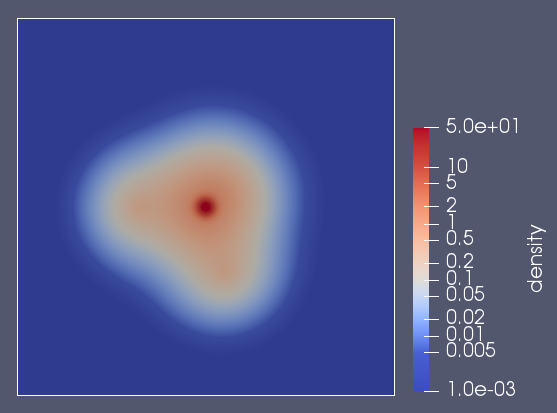
\includegraphics[width=0.48\textwidth]{h2o_density.png}
	\caption[Density plot of an optimised \ce{H2O} molecule at Hartree-Fock level]
	{Density plot of the final optimised \ce{H2O}
	Hartree-Fock geometry with a
	\ce{O-H} bond length of \unit[0.95046]{\AA} and
	a \ce{H-O-H} bond angle of $106.35^\circ$.
	A geometry optimisation in ORCA~\cite{ORCA}
	employing the same basis set
	agrees with this result within the convergence tolerance of $10^{-5}$.
	}
	\label{fig:OptimalGeometryWater}
\end{figure}
